\documentclass[english,11pt,twoside,a4paper]{article}
\usepackage[left=2cm,top=1cm,right=2cm,nohead,nofoot]{geometry}
\usepackage[utf8]{inputenc}
\usepackage{hyperref}
\usepackage{amssymb}
\usepackage{graphicx}
\usepackage{titling}
\usepackage{listings}
\newcommand{\subtitle}[1]{%
  \posttitle{%
    \par\end{center}
    \begin{center}\large#1\end{center}
    \vskip0.5em}%
}

\begin{document}
\author{
  Muona, Leo
}
\title{Mini-PL Interpreter}
\subtitle{Compilers - Project report}

\maketitle

\tableofcontents

\section{Introduction}

This document is a project report for University of Helsinki course Compilers. The subject of the project is to create an interpreter for specified Mini-PL programming language. The interpreter must scan, parse, construct an AST (abstract syntax tree) and run valid Mini-PL programs. The suggested programming language for the project was C\#, but I wrote this compiler in C++, since it is much easier to develop C++ in a Linux environment.

This report includes documentation for setup and compiling the interpreter, interpreters architectural documentation and how tokens are constructed by the scanner. Documentation also includes Mini-PL's context-free grammar used by the parser, creation of abstract syntax tree, and how errors are handled trough the program.

\section{Setup and compiling}

This Mini-PL interpreter is written in C++, in a Linux environment and has not been tested in Windows or OSX environment. Interpreter is tested in the following environment and thus have them as system requirements:

\begin{itemize}
	\item Linux operating system (kernel 3.10)
	\item GCC 4.7
	\item CMake 2.8
	\item GNU Make 3.82
\end{itemize}

It may (and probably does) also support older version of the listed software versions. In order to compile the interpreter, use the following commands in interpreters root directory:

\begin{lstlisting}[language=bash]
  $ mkdir build
  $ cd build
  $ cmake ..
  $ make
\end{lstlisting}

Now you can run the interpreter by using mpli with Mini-PL file as parameter, i.e.

\begin{lstlisting}[language=bash]
  $ ./mpli file1.mpli
\end{lstlisting}

If you want to enable debug messages, to see parse tree and AST, please modify define variable DEBUG\_MPLI to 1 in file main.cpp.

\section{Architecture}

This Mini-PL interpreter can be divided into four main components: Scanner, Parser, AST and Interpreter. Each of them have their own "jobs" and can be considered to be the four phases of the program:

\begin{itemize}
	\item Scanner: Scans character stream and constructs valid tokens that are given to the Parser.
	\item Parser: Parses the token stream into parse tree. This is used by the AST.
	\item AST: Constructs an abstract syntax tree from parse tree. This is used by the Interpreter.
	\item Interpreter: Runs the program that is described by abstract syntax tree.
\end{itemize}

If one of these components produce errors, the compiling stops and program exits without calling the next phase of the compiler.

\begin{figure}
	\begin{center}
		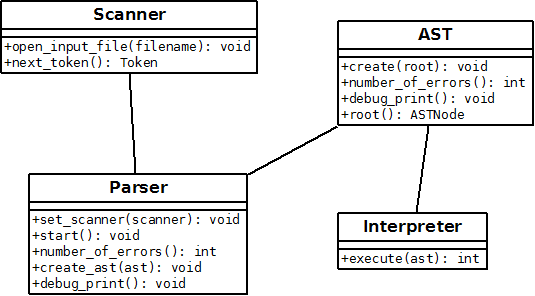
\includegraphics{class_diagram.png}
		\caption{Class diagram of the interpreter}
	\end{center}
	\label{class_diagram1}
\end{figure}

Figure~\ref{class_diagram1} shows the connections between classes, and their methods. Execution of the program goes as following:

\begin{itemize}
	\item 1. scanner.open\_input\_file(filename);
	\item 2. parser.set\_scanner(scanner);
	\item 3. parser.start();
	\item 4. parser.create\_ast(ast);
	\item 5. interpreter.execute(ast);
\end{itemize}

Parser's start()-function calls scanner's next\_token()-function as many times as there are tokens incoming. After that parser creates the AST and then interpreter executes the AST.

\section{Token construction}

Scanner creates tokens via state automaton. In Scanner's constructor, a map of state arrays are initialized that has the movement information between states. In a list below are token types as a list and how they are constructed. Some of them are not in state automaton, as token type is defined later by comparison.

\begin{itemize}
	\item IDENTIFIER: automaton: <alphabetical> ( <alpha>|<numeric>|'\_' )*
	\item INTEGER: automaton: <numeric> ( <numeric> )*
	\item STRING: automaton: '"' ( <any> )* '"'
	\item DOUBLEDOT: automaton: '.' '.'
	\item COLON: automaton: ':'
	\item INSERT: automaton: ':' '='
	\item SEMICOLON: automaton: ';'
	\item BRACKET\_RIGHT: automaton: ')'
	\item BRACKET\_LEFT: automaton: '('
	\item OP\_ADD: automaton: '+'
	\item OP\_SUBT: automaton: '-'
	\item OP\_DIVIS: automaton: '/'
	\item OP\_NOT: automaton: '!'
	\item OP\_MULT: automaton: '*'
	\item OP\_AND: automaton: '\&'
	\item OP\_LT: automaton: '<'
	\item OP\_EQ: automaton: '='
	\item KW\_VAR: check if IDENTIFIER is keyword.
	\item KW\_FOR: check if IDENTIFIER is keyword.
	\item KW\_END: check if IDENTIFIER is keyword.
	\item KW\_IN: check if IDENTIFIER is keyword.
	\item KW\_DO: check if IDENTIFIER is keyword.
	\item KW\_READ: check if IDENTIFIER is keyword.
	\item KW\_PRINT: check if IDENTIFIER is keyword.
	\item KW\_INT: check if IDENTIFIER is keyword.
	\item KW\_STRING: check if IDENTIFIER is keyword.
	\item KW\_BOOL: check if IDENTIFIER is keyword.
	\item KW\_ASSERT: check if IDENTIFIER is keyword.
	\item END\_OF\_FILE: file ended?
	\item ERROR: if token type cannot be defined.
\end{itemize}

\section{Mini-PL context-free grammar}

Parser uses the default context-free grammar that was defined by the original assignment:

\begin{lstlisting}
 <prog>   ::=  <stmts>
 <stmts>  ::=  <stmt> ";" ( <stmt> ";" )*
 <stmt>   ::=  "var" <var_ident> ":" <type> [ ":=" <expr> ] 
           |   <var_ident> ":=" <expr>  
           |   "for" <var_ident> "in" <expr> ".." <expr> "do" 
                  <stmts> "end" "for"  
           |   "read" <var_ident>  
           |   "print" <expr>  
           |   "assert" "(" <expr> ")"

 <expr>   ::=  <opnd> <op> <opnd>
           |   [ <unary_op> ] <opnd>
		   
 <opnd>   ::=  <int>
           |   <string>
           |   <var_ident>
           |   "(" expr ")"
              
 <type>   ::=  "int" | "string" | "bool"
 <var_ident> ::= <ident>
 
 <reserved keyword> ::= 
              "var" | "for" | "end" | "in" | "do" | "read" | 
              "print" | "int" | "string" | "bool" | "assert"
\end{lstlisting}

However, there are some limitations to this. <op> stands for operators '+', '-', '*', '/', '<', '=', '\&' and '!'. However integers have only following operators allowed: '+', '-', '*', '/', '<', '=' and '!'. String values have only the following operators allowed: '+', '=' and '!'. Boolean values have only '\&' and '!' allowed.

For <unary\_op> (which is '!'), only boolean value may follow it. Boolean values are produced either by '<', '=' and '!' operators or bool variables. String values can be appended with integer values by using '+' with string value as left-side operator.

There is a limitation to read statement, in which you cannot set a boolean value with read. A limitation to for statement is also applied in which you must have integer values as range. Also, analysis insists that variable used in for-in loop is defined as integer.

\section{Abstract syntax tree}

Abstract syntax tree is constructed from parse tree. This is done by removing "unnecessary" nodes and transforming other nodes into AST's node format. A list of AST node types and child node types are the following:

\begin{itemize}
	\item ROOT: possible child nodes are: INSERT, FOR\_LOOP, READ, PRINT, ASSERT and VAR\_INIT.
	\item INSERT: child nodes are in order: VAR\_ID and (OPERATOR or UNARY\_OP or VAR\_ID or CONSTANT).
	\item OPERATOR: child nodes are in order: (OPERATOR or UNARY\_OP or VAR\_ID or CONSTANT) and (OPERATOR or UNARY\_OP or VAR\_ID or CONSTANT).
	\item UNARY\_OP: child node is OPERATOR, UNARY\_OP, VAR\_ID or CONSTANT.
    \item FOR\_LOOP: child nodes are in order: FOR\_IN and FOR\_DO.
    \item FOR\_IN: child nodes are in order: VAR\_ID, (OPERATOR or VAR\_ID or CONSTANT) and (OPERATOR or VAR\_ID or CONSTANT).
    \item FOR\_DO: possible child nodes are: INSERT, FOR\_LOOP, READ, PRINT, ASSERT and VAR\_INIT.
    \item READ: child node is VAR\_ID.
    \item PRINT: child node is OPERATOR, UNARY\_OP, VAR\_ID or CONSTANT.
    \item ASSERT: child node is child node is OPERATOR, UNARY\_OP, VAR\_ID or CONSTANT.
    \item VAR\_ID: no child nodes.
    \item VAR\_INIT: child node is VAR\_ID.
    \item CONSTANT: no child nodes.
\end{itemize}

\section{Error handling}

Scanner does not handle errors. It merely just creates ERROR type tokens that it gives to Parser. Parser and AST handles errors by counting and printing them. Interpreter merely just prints errors it notices. However, certain parts of Interpreter throws std::invalid\_argument exceptions because they cannot just print and return error code, since return values from them are always "valid".

Lexical errors are identified by Scanner but printed out by Parser. Syntactical errors are identified and printed out by Parser. Semantic errors are either noticed by AST or Interpreter depending on error type. 

\section{Limitations, bugs and needed improvements}

I have noticed added the following limitation(s) to original specification:
\begin{itemize}
	\item Nested /* */ comments are not supported. C does not support them and I don't like them. However, reason them being left out was because of coding time running out.
\end{itemize}

I have noticed the following bug(s) in my interpreter:
\begin{itemize}
	\item Scanner does not notice negative integer values. This is a major bug.
	\item Scanner allows integer to start with zero. This is a major bug.
	\item Interpreter prints \n signs in strings as characters instead of line change. This is a minor bug.
\end{itemize}

Following item(s) could be to-do improvements for the interpreter:
\begin{itemize}
	\item Better error reporting: Include line number and token that causes the error.
	\item Support for multiple input files.
	\item Use only cstdio or iostream, not both.
	\item Enhance code style and algorithms.
\end{itemize}

\end{document}
